\documentclass{ctexart}

\usepackage{tikz}


\begin{document}
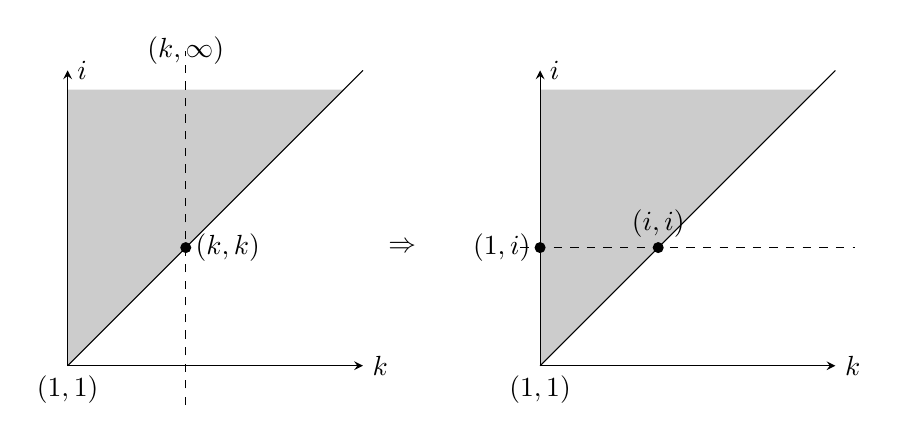
\begin{tikzpicture}[>=stealth]

\filldraw[white!80!black] (0,0) -- (3.5,3.5) -- (0,3.5);

\draw [->] (0,0)--(0,3.75) node [at end, right] {$i$};
\draw  [->]  (0,0)--(3.75,0) node [at end, right] {$k$};
\draw (0,0)--(3.75,3.75);
\draw [dashed](1.5,-.5)--(1.5,4);
\draw (0,0) [below] node {$(1,1)$};
\draw (1.5,1.5) [right] node {$(k,k)$};
\draw (1.5,4) [] node {$(k,\infty)$};
\fill (1.5,1.5) circle (2pt);

\draw node at (4.25,1.5) {$\Rightarrow$};

\filldraw[white!80!black] (6,0) -- (9.5,3.5) -- (6,3.5);
\draw [->] (6,0)--(6,3.75) node [at end, right] {$i$};
\draw  [->]  (6,0)--(9.75,0) node [at end, right] {$k$};
\draw (6,0)--(9.75,3.75);
\draw [dashed](5.75,1.5)--(10,1.5);
\draw (6,0) [below] node {$(1,1)$};
\draw (7.5,1.5) [above] node {$(i,i)$};
\draw (6,1.5) [left] node {$(1,i)$};
\fill (7.5,1.5) circle (2pt);
\fill (6,1.5) circle (2pt);



\end{tikzpicture}












\end{document}